\chapter{A brief history of molecules}\label{ch:history}

\vspace{-1.5 em}
\begin{addmargin}[-0.5cm]{0cm}
  \minitoc
\end{addmargin}
\hrule
\vspace{1.5 em}

What is Coulomb explosion imaging? A technical definition could be given, however, it is simply a decades-old technique in a long line of techniques stretching back centuries, all meant to answer a question posed by the ancient Greeks and Indians---what are the building blocks of the universe, and how do they behave?

It is easy to get stuck in the ivory tower and get lost within the trees of science, losing sight of the big picture of where your research leads.

\section{Atomism: an ancient question}

\section{Seeing molecules and saving lives}

\section{Molecular movies}
Molecular movies are of course not only of interest in physics and chemistry as a means of probing fundamental processes, but also in the biological sciences where molecular structure play a crucial role in determining the function of biomolecules such as proteins. However, the molecules of interest there are much too large to be studied by any of the previous techniques. Thus molecular movies in the biological sciences tend to be annotated computer simulations amalgamated from multiple studies. That said, they are very impressive pieces of work.

A particularly impressive movie by \citet{Cheung12} showcases the process of RNA polymerase transcription and goes on for over six minutes.

% FOCUS ON THE HISTORY OF CEI IN DETERMINING GEOMETRIES
\section{Coulomb explosion imaging}
The original CEI experiment is usually traced back to \citet{Vager89} in which the Coulomb explosion is initiated by passing a molecular beam through a thin foil. This may be because it was the first work suggesting that full molecular structures may be recovered by measuring the velocity vectors of the atomic fragments, and even reported on a non-classical molecular structure. However, previous works utilizing CEI do exist, even some that report on molecular structures \citep{Kanter79}.

Ultrashort laser pulses\footnotemark as a means of inducing Coulomb explosions made their entrance in the 1980's where they were utilized to infer molecular dynamics using covariance mapping \citep{Frasinski89}. Highly charged ion impact is another method of inducing a Coulomb explosion, and was first done in the 1990's in parallel with the development of more sophisticated coincidence mapping techniques. Since then, the laser has emerged as the more popular tool and has further developed the coincidence mapping technique. There do exist other methods of inducing Coulomb explosions, for example, single photons from a synchrotron source utilizing the Auger effect, x-ray pulses from a free-electron laser source, or electron collision.

\footnotetext{In 1987, ultrashort would be referring to \SI{0.6}{\pico\s} laser pulses \citep{Frasinski87}.}

In this section we will trace the history of CEI back to the 1970's where it started with foil-induced fragmentation. We will then follow it's development to the present day where ultrashort laser pulses are the most popular means of performing CEI. Throughout we will focus solely on the achievements of CEI in determining molecular structures, and creating molecular movies using these recovered structures\footnotemark.

\footnotetext{Much of the molecular dynamics are inferred in CEI from studying the distribution of the fragment momentum vectors (\eg through the use of Newton and Dalitz plots) and the distribution of kinetic energy carried away by each fragment. We will be focusing on the original aim of CEI, that is, to measure molecular structures.}

Interestingly, the first-ever mention of the term ``Coulomb explosion'' in the published literature comes from an unrelated study of the fine structure of singly ionized helium by \citet{Novick55}. They measured the energy difference of the $2 \, ^2 S_{1/2}$ and $2 \, ^2 P_{1/2}$ states of ionized helium as a sensitive test of quantum electrodynamics. Coulomb explosion (or space charge explosion) was the dominant ion removal mechanism which they accounted for in modeling the quenching rate\footnotemark of metastable $2 \, ^2 S_{1/2}$ ions by radio frequency radiation to describe the observed resonance lineshapes (spending two appendices on it).

\footnotetext{The term was more popular in decades past but simply means the extinction rate or loss rate of metastable ions.}

\subsection{Foil-forged images}


\begin{figure}
  \centering
  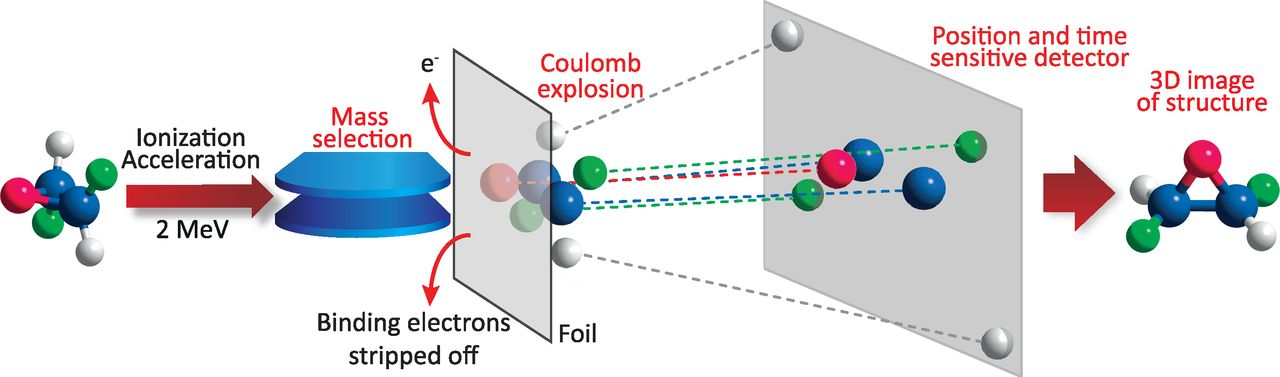
\includegraphics[width=\textwidth]{gfx/FoilExperiment}
  \caption[Schematic of a foil-induced Coulomb explosion imaging experiment.]
  {Schematic of a foil-induced Coulomb explosion imaging experiment. From \citet{Herwig13}. Reprinted with permission from AAAS.}
\end{figure}

\citet{Gaillard78} used the foil-induced Coulomb explosion to image the structure of the \ch{H3+} molecular ion, showing that it is mainly exhibits an equalaterial triangular shape in three completely different experiments\footnotemark.

\footnotetext{It is interesting to note that the experiment was repeated by separate teams at the Argonne National Laboratory, the Université Claude Bernard Lyon 1, and the Weizmann Institute of Science, then reported on in one manuscript.}

\begin{figure}
  \centering
  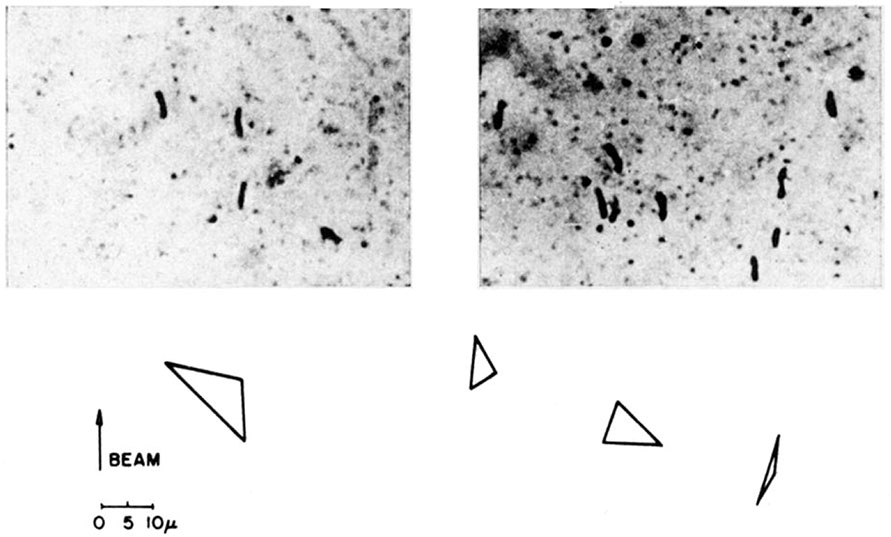
\includegraphics[width=\textwidth]{gfx/HydrogenTrimerReconstruction}
  \caption[Reconstruction of \ch{H3+} following foil-induced dissociation.]
  {Reconstruction of \ch{H3+} following foil-induced dissociation. From \citet{Gaillard78}. Reprinted with permission from APS.}
\end{figure}

CEI was first performed by \citet{Vager89} whereby the Coulomb explosion was initiated by passing a molecular beam through a thin ($\sim$\SI{30}{\angstrom}) aluminum film at high velocities ($\sim$$0.02c$). Their work was motivated by the opportunity of imaging non-classical molecular structures that more popular methods were incapble of seeing. They were also the first to suggest that measuring the velocity (or momentum) vectors of each fragment would be provide all the information required to describe the molecule's structure. Specifically for methane (\ch{CH4}), they state that the \ch{H-C-H} bond angles are preserved and that the potential energy of each \ch{C-H} pair is coverted to kinetic energy according to
$$ \frac{4e^2}{|\mathbf{r}_C - \mathbf{r}_n|} = \frac{\mu|\mathbf{V}_C - \mathbf{V}_n|^2}{2} $$
such that measurements of the asymptotic vector velocities completely defines the initial geometry of the molecule.

However, they do not perform any geometry reconstruction and report their fragment ion densities in a coordinate system defined by the asymptotic velocity of each particle, and claim that it is a direct measurement of the square of the multidimensional wave function of a many-body system.

%\begin{SCfigure}
%  \centering
%  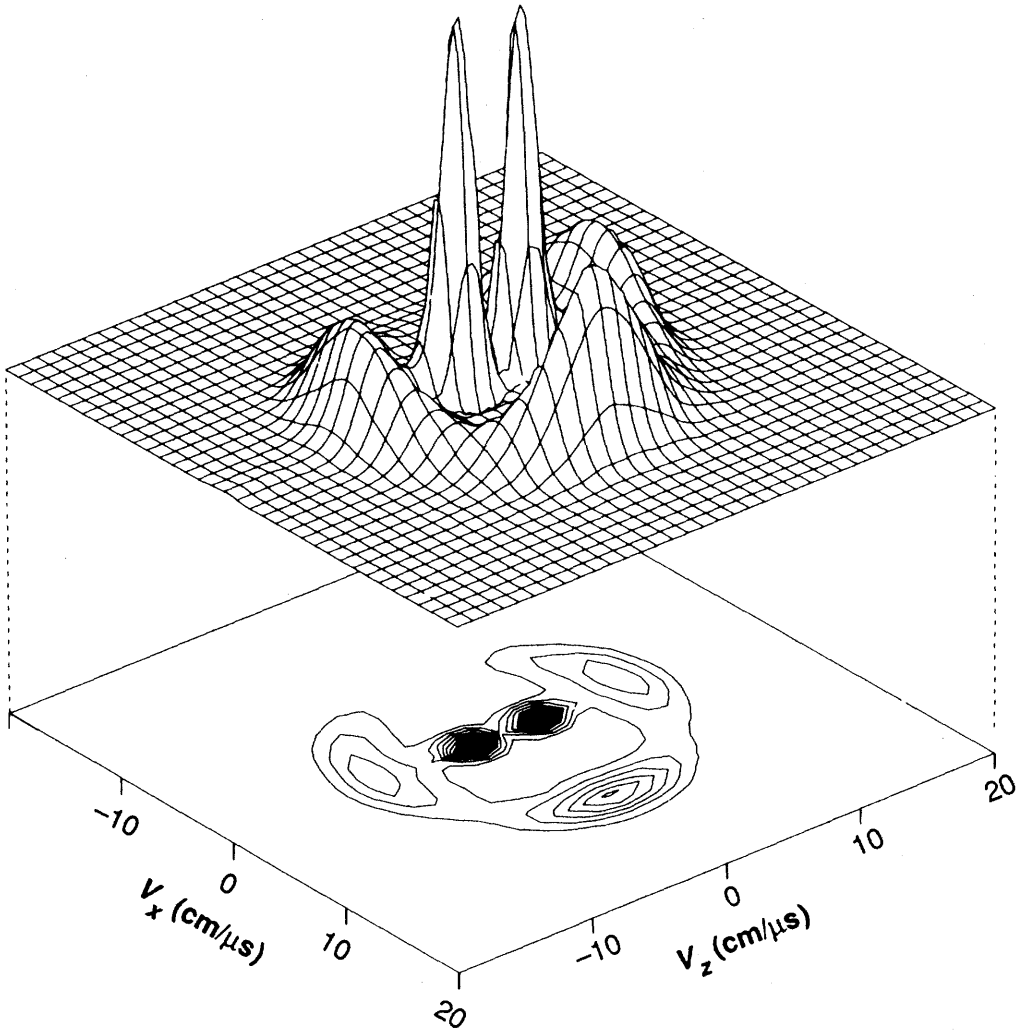
\includegraphics[width=0.5\textwidth]{gfx/VagerPseudoGeometry}
%  \caption[Reconstruction of \ch{C2H3+} following foil-induced dissociation.]
%  {Reconstruction of \ch{C2H3+} following foil-induced dissociation. From \citet{Vager89}. Reprinted with permission from AAAS.}
%\end{SCfigure}

\begin{figure}
  \centering
  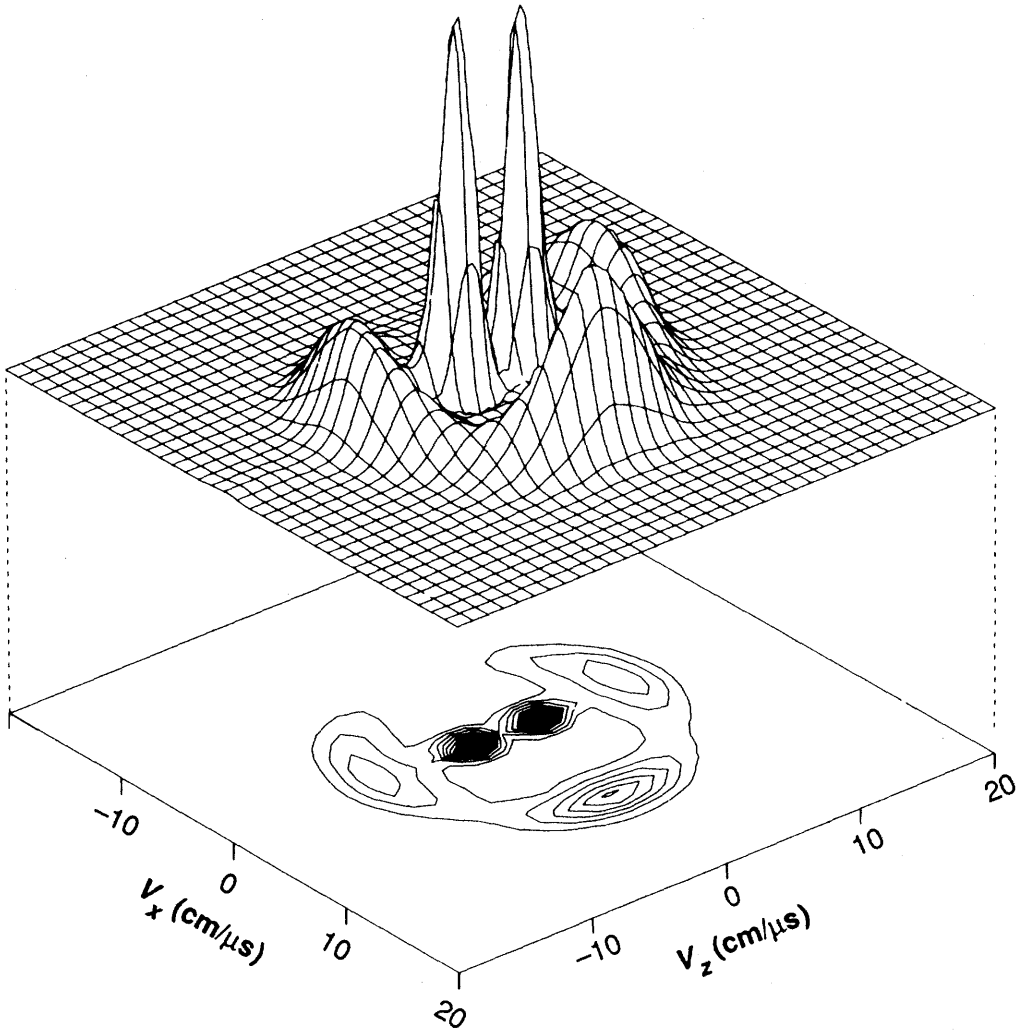
\includegraphics[width=\textwidth]{gfx/VagerPseudoGeometry}
  \caption[Reconstruction of \ch{C2H3+} following foil-induced dissociation.]
  {Reconstruction of \ch{C2H3+} following foil-induced dissociation. From \citet{Vager89}. Reprinted with permission from AAAS.}
\end{figure}

One drawback of initiating Coulomb explosions using a thin foil is that a molecular beam must be prepared.

\subsection{Fragmentation by highly charged ion impact}

\subsection{Laser-induced dissociation}
\citet{Legare05structure,Legare05dynamics} was the first to use ultrashort laser pulses to induce Coulomb explosion and report on molecular structures and dynamics. To obtain the structures, they assume the explosion proceeds under a purely Coulombic potential and use optimization methods to make guesses at the structure that most accurately reproduces the observed data consistent with minimizing a least-squares objective function. Unfortunately they provide very minimal information regarding their methods and there is a complete lack of discussion acknowledging the shortcomings of this method\footnotemark. Using 8 fs laser pulses they report on the structure of \ch{D2O} and \ch{SO2} \citep{Legare05structure}. They also claim to have imaged vibrating \ch{D2+} and dissociating \ch{SO2^{2+}} and \ch{SO2^{3}} however they provide no more than a couple of dissociation frames and infer the transient \ch{D2+} bond length from kinetic energy release ratios as a function of pump-probe time delay \citep{Legare05dynamics}.

\footnotetext{The main shortcomings being degenerate solutions and the fact that they employ convex optimization methods to a problem that is not convex. It is not clear if they even knew about these issues.}

\index{Classical imaging formula}
\index{Coulomb explosion imaging!Classical imaging formula}
Surprisingly, an attempt was made to arrive at an analytical solution for calculating geometries from measured momentum data. \citet{Nagaya04} were able to derive a so-called classical imaging formulas giving the position wavefunction squared for the Coulomb explosion of a diatomic molecule and a linear triatomic molecule\footnotemark. They treat the cases of symmetric and asymmetric Coulomb explosion.

\footnotetext{They seem to have worked hard to find an analytical solution but their unsaid conclusion seems to be that it is an intractable problem and their group went silent on this problem.}

\citet{Gagnon08} reported the reconstruction of dichloromethane (\ch{CH2Cl2}) using a home-made \footnotemark stochastic-based simulated annealing algorithm that globally optimizes the molecular spatial configuration. They discuss uncertainties but are only able to obtain the structure in five cases.

\footnotetext{There is nothing wrong with writing your own code here but nonconvex optimization algorithms are tricky to get right and the reliance should be on professional code.}

\index{Lookup table}
The best effort so far has probably been the one by \citet{Kunitski15} in which they use a lookup table approach to image the elusive Efimov state of the helium trimer.